\documentclass{article}
\usepackage{amssymb,amsmath}
\usepackage{ifxetex,ifluatex}
\ifxetex
  \usepackage{fontspec,xltxtra,xunicode}
  \defaultfontfeatures{Mapping=tex-text,Scale=MatchLowercase}
\else
  \ifluatex
    \usepackage{fontspec}
    \defaultfontfeatures{Mapping=tex-text,Scale=MatchLowercase}
  \else
    \usepackage[utf8]{inputenc}
  \fi
\fi
\usepackage{ctable}
\usepackage{float} % provides the H option for float placement
\usepackage{graphicx}
% We will generate all images so they have a width \maxwidth. This means
% that they will get their normal width if they fit onto the page, but
% are scaled down if they would overflow the margins.
\makeatletter
\def\maxwidth{\ifdim\Gin@nat@width>\linewidth\linewidth
\else\Gin@nat@width\fi}
\makeatother
\let\Oldincludegraphics\includegraphics
\renewcommand{\includegraphics}[1]{\Oldincludegraphics[width=\maxwidth]{#1}}
\ifxetex
  \usepackage[setpagesize=false, % page size defined by xetex
              unicode=false, % unicode breaks when used with xetex
              xetex]{hyperref}
\else
  \usepackage[unicode=true]{hyperref}
\fi
\hypersetup{breaklinks=true, pdfborder={0 0 0}}
\setlength{\parindent}{0pt}
\setlength{\parskip}{6pt plus 2pt minus 1pt}
\setlength{\emergencystretch}{3em}  % prevent overfull lines
\setcounter{secnumdepth}{0}

\title{Outlier test}
\author{(Username not set) (E-mail address not set)}
\date{2011--04--26 20:25 CET}

\begin{document}
\maketitle

\subsection{Description}

This template will check if provided variable has any outliers.

\subsubsection{Boxplot}

\begin{figure}[htbp]
\centering
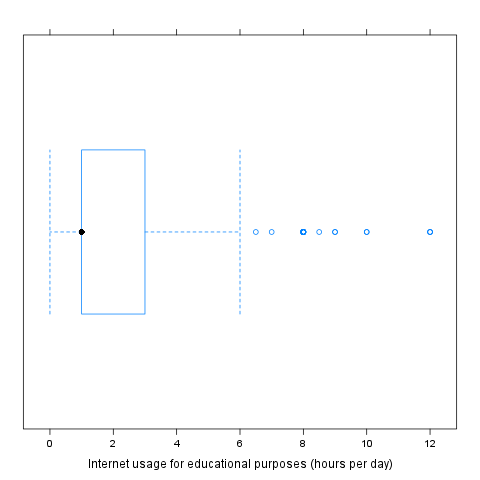
\includegraphics{7e4826ae32ce6332453510e91fb95335.png}
\caption{}
\end{figure}

\subsubsection{Lund test}

It seems that 5 extreme values can be found in ``Internet usage for
educational purposes (hours per day)''. These are: 10, 10, 12, 12, 12.

\paragraph{Explanation}

The above test for outliers was based on \emph{lm(1 \ensuremath{\sim}
it.edu)}:

\ctable[pos = H, center, botcap]{lllll}
{% notes
}
{% rows
\FL
 & \textbf{Estimate} & \textbf{Std. Error} & \textbf{t
value} & \textbf{Pr(\textgreater{}\textbar{}t\textbar{})}
\ML
(Intercept) & 2.06 & 0.08 & 26.92 & 0.00
\LL
}

\paragraph{The residuals returned:}

--0.0308, 2.9119, --0.2760, --0.5212, --0.5212, --0.7665, --1.0117,
--0.2760, --0.5212, 1.4406, --0.5212, 0.9501, 3.8929, --0.0308,
--0.5212, --0.7665, --0.0308, 1.4406, --0.5212, 0.4597, 1.9310,
--0.5212, 0.9501, --0.5212, 0.9501, --0.0308, 0.4597, --0.7665, 0.9501,
--0.7665, --0.5212, --0.5212, --0.5212, 1.4406, 3.4024, --0.5212,
--0.5212, --0.2760, --0.5212, --0.5212, --0.7665, --0.7665, 0.9501,
0.4597, --0.5212, 1.4406, 1.4406, --0.5212, --0.7665, 0.4597, --0.0308,
1.4406, --0.5212, 2.9119, 0.4597, --0.7665, 1.4406, 0.9501, 1.4406,
--0.7665, --0.5212, --0.0308, --0.7665, --0.5212, 0.4597, --0.7665,
0.9501, --0.7665, --0.5212, --0.7665, --0.0308, --0.5212, 0.4597,
0.4597, --0.0308, --0.7665, --1.0117, --0.7665, --0.5212, --0.5212,
--0.2760, --0.7665, --0.7665, 2.9119, --0.0308, 2.9119, 0.4597,
--0.0308, --0.5212, --0.5212, --0.2760, --0.7665, 0.9501, --0.5212,
--0.0308, --0.7665, 0.7049, --0.5212, --0.7665, --0.5212, 0.2144,
--0.0308, --0.0308, --0.0308, --1.0117, --0.7665, --0.2760, 2.9119,
--1.0117, 1.1954, 0.9501, 2.9119, --0.2760, --0.0308, 0.9501, --0.7665,
--1.0117, --0.7665, --0.5212, 0.4597, --0.7665, --1.0117, 2.9119,
--0.5212, --0.7665, --0.5212, --0.7665, --0.5212, --1.0117, --0.5212,
2.4215, --0.5212, --0.5212, 1.4406, 0.2144, 0.2144, 0.9501, 0.4597,
0.2144, --0.2760, 0.9501, 1.9310, --0.7665, 0.2144, --0.0308, --0.5212,
--1.0117, --1.0117, --0.0308, --0.0308, --0.0308, --0.7665, --0.5212,
--0.5212, --0.5212, --0.5212, --0.5212, --1.0117, --0.5212, 0.4597,
--0.0308, --0.5212, 0.4597, --0.7665, 0.2144, 1.4406, 1.4406, --1.0117,
1.4406, 0.9501, --0.7665, --0.5212, --0.7665, --0.7665, --0.0308,
--0.5212, 0.4597, --0.0308, --0.5212, --0.5212, --0.0308, --0.7665,
--0.5212, 2.9119, --0.7665, --0.7665, --0.5212, --0.7665, --0.0308,
--0.0308, --0.7665, --0.5212, --0.5212, --1.0117, --0.5212, --0.5212,
0.4597, --0.0308, 0.4597, --0.5212, --0.5212, --1.0117, --1.0117,
--0.0308, --1.0117, --0.5212, --0.5212, 0.9501, --0.7665, 2.9119,
--0.5212, --0.0308, --1.0117, 1.4406, 0.4597, --0.5212, --0.0308,
--0.7665, --0.5212, --0.5212, --1.0117, --0.7665, --0.7665, --1.0117,
--0.7665, --0.5212, 0.4597, --0.0308, --0.0308, --1.0117, --0.7665,
--0.5212, --0.0308, --0.5212, --0.0308, --1.0117, 0.9501, 0.4597,
--0.0308, --0.0308, 0.4597, --0.5212, --1.0117, 2.9119, --0.0308,
--0.5212, 0.9501, --0.5212, --0.0308, 3.4024, 0.4597, --0.5212,
--0.5212, --0.5212, --0.0308, --0.7665, --0.5212, --0.7665, --0.7665,
--0.5212, --1.0117, --0.5212, 0.4597, --0.0308, --0.5212, --0.0308,
--0.5212, --0.5212, 0.4597, --1.0117, --0.0308, --0.7665, 3.8929,
0.4597, --0.7665, 0.4597, --1.0117, --0.7665, --0.7665, --0.0308,
--0.2760, --0.0308, --0.7665, --0.7665, --0.0308, 0.4597, --0.5212,
--0.5212, --0.5212, --0.0308, --0.2760, --0.5212, --0.0308, 1.9310,
1.9310, 2.9119, --0.7665, 0.4597, 4.8738, --0.7665, 1.4406, 2.9119,
--0.5212, 0.9501, --1.0117, --0.5212, 2.9119, --0.0308, 2.9119,
--0.5212, 0.9501, 0.9501, 0.4597, --0.5212, --0.2760, --0.5212,
--0.7665, --0.5212, --0.5212, --0.5212, --0.5212, 0.4597, --0.7665,
1.4406, --0.5212, --0.0308, --0.0308, --0.0308, --0.5212, --0.5212,
--0.7665, 1.9310, --0.5212, --0.0308, --0.5212, --1.0117, --0.5212,
0.4597, --0.7665, --0.5212, 0.4597, --0.5212, 4.8738, --0.5212,
--0.2760, --0.5212, 0.4597, --1.0117, --0.7665, --0.5212, 2.9119,
1.4406, --0.0308, --0.2760, 1.9310, 2.9119, --0.5212, 2.9119, 0.4597,
--0.5212, 0.9501, 0.2144, --0.0308, --0.5212, --1.0117, --1.0117,
1.6858, 0.2144, --0.5212, --0.5212, --0.2760, --1.0117, --0.5212,
--1.0117, --0.5212, --0.7665, --0.5212, 0.4597, --0.0308, --1.0117,
--0.0308, 0.4597, 0.4597, 0.4597, --0.5212, --0.5212, 2.9119, --0.5212,
--1.0117, 2.9119, --1.0117, --0.5212, 0.4597, --1.0117, 1.4406,
--0.0308, 0.9501, --1.0117, 2.9119, --0.5212, --0.7665, 0.9501,
--0.0308, --0.5212, 0.2144, --0.0308, --0.5212, --0.7665, 4.8738,
1.9310, 0.9501, --0.0308, 0.9501, 1.1954, 0.4597, --0.7665, --0.7665,
--1.0117, 0.9501, 2.9119, 0.4597, 1.4406, 2.9119, --0.5212, 0.4597,
1.4406, --1.0117, --0.0308, 0.4597, --0.0308, 1.9310, --0.5212,
--0.5212, 1.4406, --0.0308, --0.5212, --0.7665, --0.5212, --0.5212,
0.2144, --0.5212, --0.5212, --0.5212, --0.5212, --0.0308, --0.7665,
--0.0308, 0.9501, --0.5212, 0.4597, --0.0308, --0.7665, --0.0308,
--0.5212, --0.5212, --0.5212, --0.0308, --0.5212, --0.5212, --0.7665,
--0.5212, --0.2760, --0.7665, --0.0308, --0.7665, --0.5212, 1.4406,
--1.0117, 0.9501, --0.0308, --0.7665, --0.7665, --0.5212, --0.5212,
--0.5212, --0.5212, --0.0308, --0.7665, --0.5212, --0.5212, --0.5212,
--0.5212, 0.7049, --0.0308, --0.5212, 0.4597, --0.0308, --0.5212,
--0.7665, --0.5212, --0.7665, --1.0117, --0.0308, --0.5212, --0.0308,
0.9501, --0.5212, --0.5212, --0.0308, --0.7665, --0.5212, 0.2144,
--0.2760, --0.0308, --0.5212, --0.7665, --0.5212, --0.0308, --0.0308,
--0.5212, --0.0308, --0.5212, 1.9310, --0.2760, 1.9310, --0.5212,
--0.5212, --0.2760, --0.5212, --0.0308, 0.4597, --0.7665, --0.5212,
0.4597, 0.9501, --0.0308, 1.4406, --0.5212, 0.4597, 0.4597, --0.5212,
--0.2760, 0.2144, 1.4406, --0.2760, 1.4406, --0.0308, 0.4597, 1.4406,
--0.5212, --0.2760, --0.5212, --0.5212, --0.0308, --0.5212, --0.0308,
--0.7665, --0.7665, --0.7665, --0.5212, --0.7665, --0.5212, --0.2760,
--0.0308, 0.4597, 0.9501, --1.0117, --0.2760, 1.9310, 1.9310, --0.5212,
--0.5212, 0.4597, --0.5212, 0.9501, --0.5212, --1.0117, --0.0308,
0.9501, --0.7665, --0.0308, 0.9501, --0.5212, --0.2760, 2.1763,
--0.0308, 0.9501, 0.4597, 1.4406, 0.2144, --0.7665, --0.5212, --1.0117,
--0.0308, 0.4597, --0.7665, --1.0117, --1.0117, --0.5212, --0.5212,
--0.0308, --0.5212, --0.2760, --1.0117, --0.0308, 0.4597, --0.7665,
--0.5212, --0.5212, --0.5212, --0.0308, --0.5212, --0.5212, 0.4597,
--0.5212, --1.0117, --1.0117, 0.4597, --0.2760, --0.5212, 1.9310,
--0.0308, --0.5212, --1.0117, --0.5212, --0.7665, --1.0117, 0.9501,
0.9501, 1.4406, --0.7665, --0.5212, --0.5212, --0.0308, 1.4406,
--1.0117, 0.4597, --0.5212, 1.4406, 0.4597, --0.7665, --0.5212,
--0.7665, --1.0117, --0.7665, --0.7665, --0.0308, --1.0117, 0.2144,
0.4597, 2.9119, 0.4597, --0.7665, --0.7665, --0.0308, 0.2144, --0.0308,
0.4597, --0.5212, 0.2144, 2.9119, --1.0117, --0.5212, --0.5212, 1.4406,
--0.5212, --0.2760, --1.0117, --0.0308, --0.0308, --0.0308, 0.2144,
--1.0117, 0.4597, --0.5212, --0.7665, --0.5212, --0.7665, --0.0308,
--0.5212, 0.4597, --0.5212, --1.0117, --0.0308, --0.0308, --0.0308,
--0.0308, 1.4406, 0.9501, --1.0117, --0.0308, 1.4406, --0.5212,
--0.0308, 0.4597, --0.5212, 1.4406, 0.4597, --0.5212, 0.4597, --0.5212,
--0.7665, --0.5212, --1.0117, --0.7665, --0.0308, --0.5212, --0.7665,
--0.0308, --0.7665, --0.5212, --0.5212, --0.7665, 2.9119, 3.1572,
--1.0117, --1.0117, --0.7665, --0.5212

\paragraph{References}

\begin{itemize}
\item
  Lund, R. E. 1975, ``Tables for An Approximate Test for Outliers in
  Linear Models'', Technometrics, vol.~17, no. 4, pp.~473--476.
\item
  Prescott, P. 1975, ``An Approximate Test for Outliers in Linear
  Models'', Technometrics, vol.~17, no. 1, pp.~129--132.
\end{itemize}
\subsubsection{Grubb's test}

Grubbs test for one outlier shows that highest value 12 is an outlier
(p=0.0003).

\paragraph{References}

\begin{itemize}
\item
  Grubbs, F.E. (1950). Sample Criteria for testing outlying
  observations. Ann. Math. Stat. 21, 1, 27--58.
\end{itemize}
\subsubsection{Dixon's test}

chi-squared test for outlier shows that highest value 12 is an outlier
(p=0).

\paragraph{References}

\begin{itemize}
\item
  Dixon, W.J. (1950). Analysis of extreme values. Ann. Math. Stat. 21,
  4, 488--506.
\end{itemize}

\end{document}
